\documentclass[a4paper,12pt]{article}
\usepackage{tkz-euclide}
\usepackage{gensymb}
\usepackage[utf8]{inputenc}
\usetikzlibrary{math}
\usepackage{graphicx}
\title{ASSIGNMENT-7}
\author{SENANI SADHU}
\date{\today}
\begin{document}
		\maketitle
	\pagenumbering{roman}
	\newpage
	\section{Draw a circle of radius 3 and any two of its
		diameters. Draw the ends of these diameters.
		What figure do you get?}
	\subsection{Solution:-}
	Given a circle with radius 3, also having its centre as O.\\
	 Let AC and BD be two diameters of this circle. When we join the ends of these diameters, a quadrilateral ABCD is formed.
	As we know that the diameters of a circle are equal in length, therefore, the quadrilateral so formed will have its diagonals of equal length.
	Also, OA=OB=OC=OD radius r=3 and if a quadrilateral has its diagonals of same length which are bisecting each other, then it will be a rectangle.\\
	a=c and b=d where a,b,c,d are sides of rectangle.\\
	x=y=6(Diameter of circle.)
	\begin{center}
		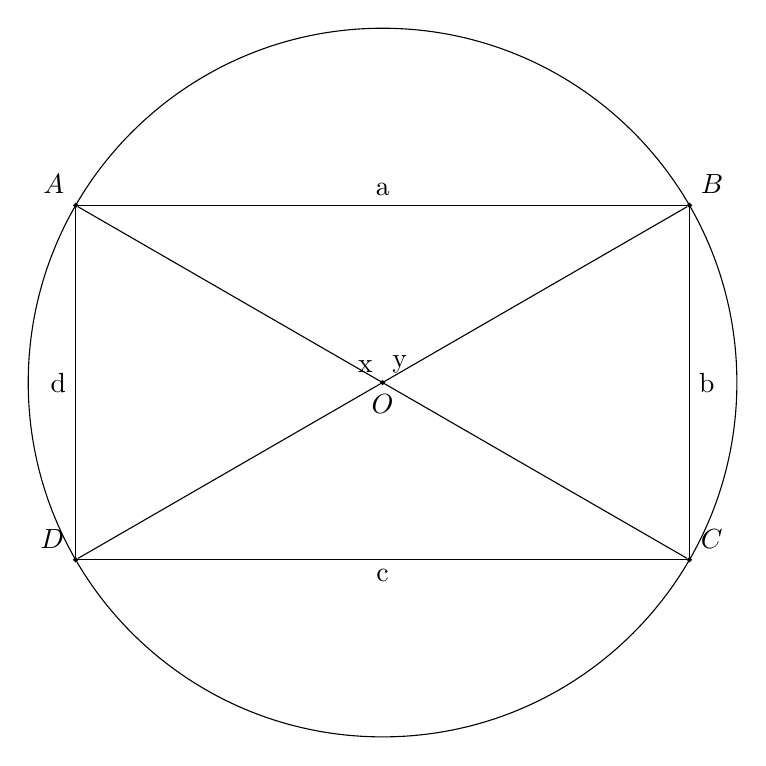
\begin{tikzpicture}
			[scale=1.5,>=stealth,point/.style={draw,circle,fill = black,inner sep=0.5pt},]
			\tikzmath{\t1=30; \t2=-150; \t3=150; \t4=-30; }
			\draw (0,0) circle(3cm);
			\node (O) at (0, 0)[point,label=below :$O$] {};
			\node (A) at ({\t3}:3)[point,label=above left:$A$]{};
			\node (B) at ({\t1}:3)[point,label=above right:$B$]{};
			\node (D) at ({\t2}:3)[point,label=above left:$D$]{};
			\node (C) at ({\t4}:3)[point,label=above right:$C$]{};
			\draw (A) --  node[above] {$\textrm{a}$}(B) --  node[right] {$\textrm{b}$}(C) --  node[below] {$\textrm{c}$}(D) --  node[left] {$\textrm{d}$}(A);
			\draw (A) -- node[above left] {$\textrm{x}$}(C);
			\draw (B) -- node[above right] {$\textrm{y}$}(D);
			
	\end{tikzpicture}
	\end{center}
\subsection{Output of Python Code:-}
\begin{figure}[htp]
	\centering
	\includegraphics[width=10cm]{new1.png}
	\caption{Fig generated using python}
\end{figure}
\end{document}